%
% chapter5.tex
%

\chapter{Experiments}\label{cha:experiments}
Paul Raatschen has performed a study\cite{raatschen:ipc} concluding that the original Fail2ban process can be improved upon.
It was determined that especially with many clients, Fail2ban struggled to keep up with high incoming traffic rates.
To remedy this issue, a more performant program, Simplefail2ban, was implemented and measured.
An increase in performance was evident.
Simplefail2ban supported two modes of IPC (TODO: Abbreviation).
The disk mode was akin to traditional file logging, while the shared memory approach would use a shared memory section to exchange data between processes.
A direct comparison between the already outlined socket approach and previously supported IPC (TODO: Abbreviation) types necessitates the measurements in this chapter.

The following chapter details the conducted measurements, outlining specifics according to Jain's
``The Art of Computer Systems Performance Analysis: Techniques For Experimental Design, Measurement, Simulation, and Modeling, NY\@: Wiley''\cite{jain:measurement} chapter 2.2.

\section{Test environment}
Two machines, both identical in hardware and software, were used in these experiments.
The first machine, the device under test (DUT) (TODO: Abbreviation), ran Simplefail2ban and a test application responsible for receiving incoming traffic and reporting clients.
The second machine generated and sent traffic, consisting of both valid and invalid traffic, to the DUT (TODO: Abbreviation) using TRex.

\begin{table}[b!]
    \renewcommand{\arraystretch}{1.5}
    \caption[Testbed specs]{Table of Hardware and Software parameters of the testbed. Both machines are identical.
    The first machine serves as the DUT, the second machine generates traffic to be sent to the DUT (TODO: Abbreviation, also for the table below) via TRex.}\label{tab:specs}
    \centering
    \small
    \begin{tabular}{ll}
        \toprule
        \multicolumn{2}{l}{\textbf{Hardware}} \\ \midrule
        CPU     & 16 $\times$ Intel(R) Xeon(R) Silver 4314 CPU @ 2.40GHz \\
        NIC     & Mellanox Technologies MT2892 Family [ConnectX-6 Dx] \\
        RAM     & 128 GB \\ \bottomrule

        \multicolumn{2}{l}{\textbf{Software}} \\ \midrule
        OS          & Debian GNU/Linux 11 \\
        Kernel      & 5.10.0-28-amd64 x86\_64 \\
        NIC Driver  & mlx5\_core; Version 5.8-2.0.3 \\
        TRex        & 2.99 (Stateless) \\ \bottomrule
    \end{tabular}
\end{table}

\section{Experimental design}
In his thesis\cite{raatschen:ipc} Paul Raatschen showed that the shared memory mode of Simplefail2ban outperforms the traditional Fail2ban.
However, it remains unclear if the implementation of this IPC type is more performant than other alternatives.
Specifically, the possibility of using Unix domain sockets as a mode of inter-process communication was not explored.
The following experiments enable a direct comparison between the two IPC types.

\noindent
In general, the experiments consist of two participants and a one-sided data exchange.
The device under test (DUT) (TODO: Abbreviation), or more specifically the application udp\_server, receives a stream of both wanted and unwanted data.
Identifying desired traffic is done by analyzing the message payload.
This is a crude and unrealistic approach to filtering malicious communication requests.
Such a simplification allows the application udp\_server to quickly generate log messages.
Since the goal of this study is to determine the most efficient IPC type for Simplefail2ban, this abstraction does not diminish the findings of this thesis.

\noindent
To compare the differing IPC (TODO: Abbreviation) types, a set of performance metrics needs to be established:

\bigskip
\noindent
\textbf{Performance metrics}
\begin{itemize}
    \item Total number of unwanted requests dropped (number of packets)
    \item Total number of unwanted requests dropped, relative to the total amount of unwanted requests send (percentage)
    \item Number of log messages processed by Simplefail2ban, relative to the number of log messages sent by the test server (percentage)
    \item Central Processing Unit (CPU) utilization of Simplefail2ban (seconds of CPU time)
\end{itemize}
Higher is better for the first three metrics.
The last metric should be minimized for the DUT (TODO: Abbreviation) so its services are continually provided to valid clients.

\bigskip
\noindent
The fixed parameters for each of the experiments are the following\@:

\bigskip
\noindent
\textbf{Fixed parameters}
\begin{itemize}
    \item Hardware and Software parameters of the testbed (TODO: Abbreviation) in this table\@:
    \begin{itemize}
        \item CPU\@: 16 cores, no hyper-threading enabled
        \item Network Interface Card (NIC)\@: Maximum transfer unit, 1500 bytes
        \item TRex\@: One interface, 30 threads
    \end{itemize}
    \item Number of entries in eBPF maps for IPv4 \& IPv6\@: 1,000,000
    \item Number of receiving threads used by udp\_server\@: 16
    \item Duration of measurement\@: 300 Seconds
    \item Amount of valid traffic sent \@: 50,000 PPS
    \item Number of clients sending valid traffic\@: 254
    \item \textbf{Simplefail2ban} parameters\@:
    \begin{itemize}
        \item Number of hash table bins used\@: 6,000,011
        \item Ban threshold for clients\@: 3
        \item Ban time for clients\@: 30 seconds
        \item Enabling the Regex Matching feature of Simplefail2ban (the current implementation does not ban clients correctly when disabled)
        \item For \textbf{shared memory} specifically\@:
        \begin{itemize}
            \item Number of banning threads used\@: 16
            \item Line count for the shared memory buffer segments\@: 1,000,000
            \item Segment count for the shared memory buffer\@: 16
            \item Overwrite feature enabled
            \item Workload stealing feature disabled
        \end{itemize}
        \item For \textbf{sockets} specifically\@:
        \begin{itemize}
            \item Number of banning threads used\@: 16
            \item Number of sockets\@: Same as number of reader processes
            \item Using default path to sockets created by the application\@: tmp/
            \item Using default socket receive and send buffer size configured on the system\@: 212992 Bytes
        \end{itemize}
        \item For \textbf{disk} specifically\@:
        \begin{itemize}
            \item Number of banning threads used\@: 1 (disk mode only supports one banning threads)
            \item Buffer size for uring\_getlines\@: 2048
        \end{itemize}
    \end{itemize}
\end{itemize}

\bigskip
\noindent
The factors, or variable parameters, during these experiments were the following\@:

\bigskip
\noindent
\textbf{Factors and their levels}
\begin{itemize}
    \item Effects of differing amount of invalid traffic sent: 100k, 1m, 10m, 20m, 30m PPS
    \item Effects of differing number of clients sending invalid data: 65,534 and 131,068
    \begin{itemize}
        \item Range used for 65,534 clients: 10.4.0.1 to 10.4.255.254 resulting in clients stemming from 256 subnets (using offset\_fixup of 5 for IPv6 in TRex script).
        \item Range used for 131,068 clients: 10.4.0.1 to 10.5.255.252 resulting in clients stemming from 512 subnets (using offset\_fixup of 5 for IPv6 in TRex script).
        \item When using the IPv4/IPv6 IP stack, the range for 65,534 client is being used twice to generate both a IPv4 and IPv6 stream.
    \end{itemize}
    \item IP stack: IPv4, IPv6 and IPv4/IPv6 mixed
    \item Differing IPC type\@: DISK, SHM, SOCK
    \item For shared memory specifically:
    \begin{itemize}
        \item No 2nd Reader/ Enabling 2nd Reader
    \end{itemize}
    \item For sockets specifically:
    \begin{itemize}
        \item No 2nd Reader/ Enabling 2nd Reader
    \end{itemize}
\end{itemize}

\bigskip
\noindent
To generate the traffic being sent to the DUT, TRex scripts are used.
These scripts provide the option to modify the sent traffic according to the factors outlined above. TODO: Add path in repo for these scripts
During these measurements, adapted versions of Paul Raatschens\cite{raatschen:ipc} scripts were used.
To measure most performance metrics, an adaptation of the xdp\_ddos01\_blacklist\_cmdline program was used.
This application originally stems from Florian Mikolajczak master's thesis\cite{mikolajczak:ebpf} and routinely polls the number of dropped and passed packets from a specific eBPF map.
It was modified by Paul Raatschen to output values as a csv file.
The polled eBPF map is ultimately used by Simplefail2ban to ban clients.
CPU time was measured via the command top.

\section{Replicative experiments}
Software version changes warrant remeasurement of the shared memory and disk IPC (TODO: Abbreviation) mode for Simplefail2ban.
These will also be used to evaluate the newly implemented socket mode.

\subsection{Experiment 1a: Replication of Simplefail2ban Logfile}
It has already been shown that the disk mode of Simplefail2ban is outperformed by the shared memory mode.
Pure IPv4, IPv6 and a mixed IPv4/IPv6 IP stack will be used.
File logging is expected to perform worse than the other IPC (TODO: Abbreviation) modes discussed in this thesis.
In total, 25 unique measurements were conducted for this experiment.

\subsection{Experiment 1b: Replication of Simplefail2ban Shared Memory}
The newly implemented socket approach is intended to be a valid alternative to the shared memory mode of Simplefail2ban.
To enable a direct comparison, measurements for the shared memory mode need to be done under high loads, since with lower loads both the socket and shared memory mode are suspected to be performant enough.
All levels of invalid traffic rates are measured individually.
Again, either a pure IPv4, IPv6 or mixed IPv4/IPv6 IP stack is utilized.
The most performant features will be used, meaning overwrite is enabled and workload stealing is disabled.
No second reader process is being employed here.
In total, 25 unique measurements were conducted for this experiment

\section{Measuring the socket API}
In the following section thorough variations of factors and their levels are used to conclude if the socket mode is reliable.
Also, heavy workloads are employed to determine how the socket mode performs in worst case scenarios.
This will enable a direct comparison between socket and shared memory mode.
The data flow in the DUT can be seen in \ref{fig:socket:measurement}.

\begin{figure}[h!]
    \centerline{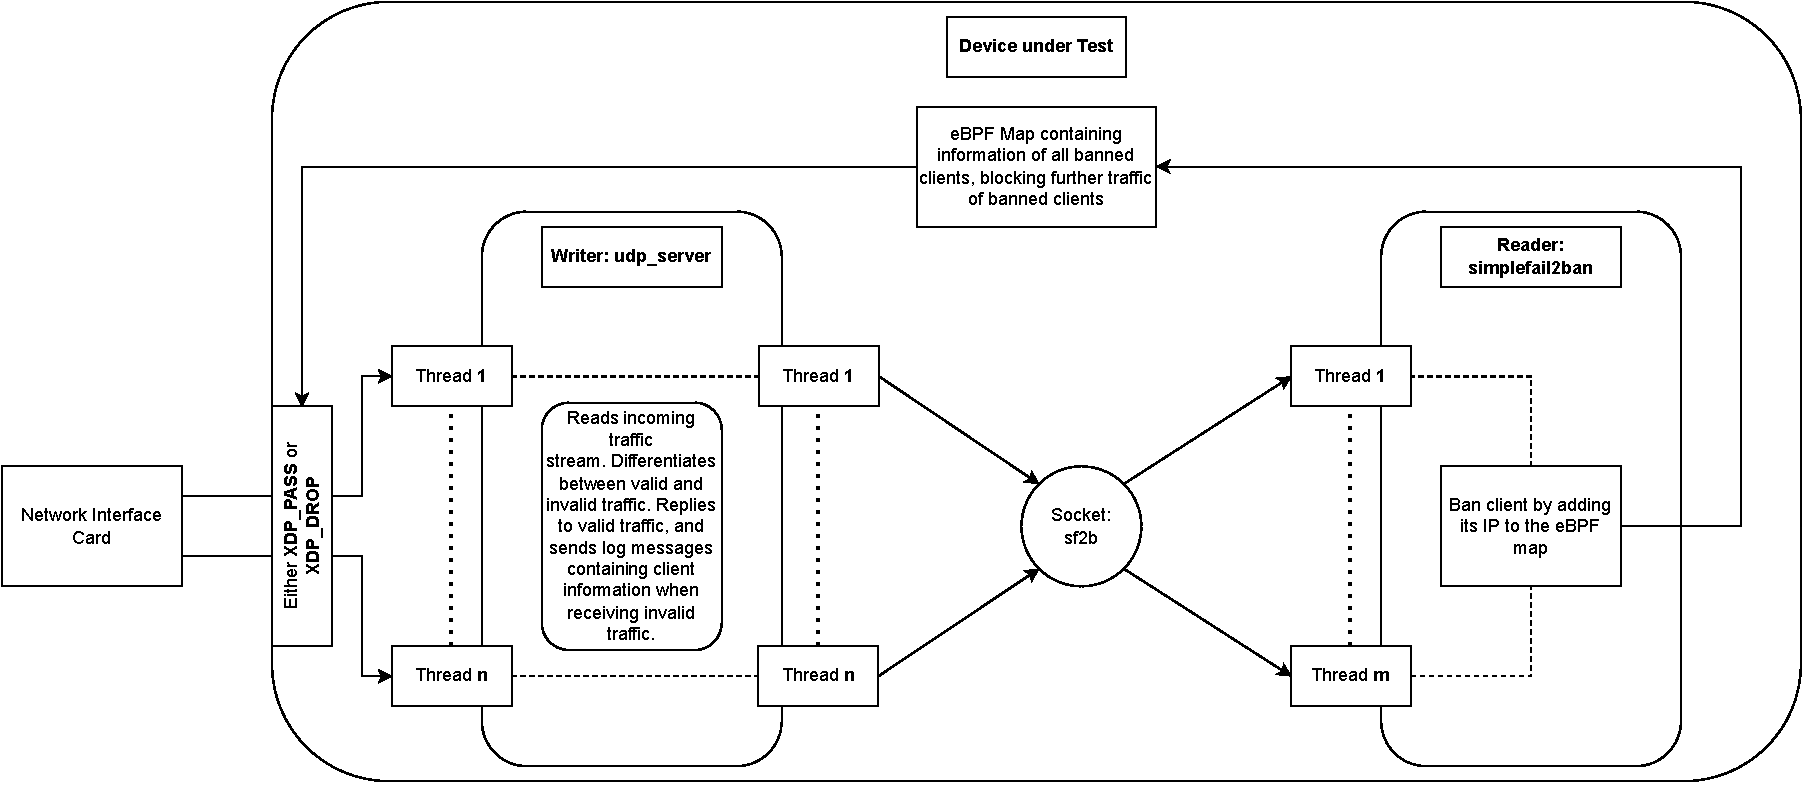
\includegraphics[width=1.2\textwidth]{images/MeasurementArchitecture.pdf}}
    \caption[DUT during socket measurements]{
        The graphic displays the data flow (left to right) on the DUT when enabling sockets as the IPC type.
        A packet can either be passed (XDP\_PASS) or to the kernel or dropped (XDP\_DROP) before ever reaching it.}
	\label{fig:socket:measurement}
\end{figure}


\subsection{Experiment 2: Simplefail2ban Sockets}
To establish a baseline for the performance of the socket mode all factors are set to all possible levels in every combination.
The only exception being the possibility of using a second reader process, which will have its own section later.
In total, 25 unique measurements were conducted for this experiment.

\subsection{Experiment 3a: Replication of Simplefail2ban Shared Memory with 2nd Reader}
In order to later compare the socket mode and its option to have a second reader, a baseline measurement needs to be established.
This experiment will be performed with 131,068 clients sending invalid data only and no pure IPv4 or IPv6 IP stack.
Again, the overwrite feature is enabled while workload stealing is disabled.
In total, 5 unique measurements were conducted for this experiment.

\subsection{Experiment 3b: Simplefail2ban Sockets with 2nd Reader}
This experiment closely mirrors the experiment 3a.
A total of 131,068 clients will send invalid data to the DUT with no pure IPv4 or IPv6 IP stack.
The shared memory mode inherently supports the possibility of adding a second reader to the shared memory section to read log messages.
There is no such inherent support in the socket mode.
Instead in its current implementation, another read process can be started which will then be assigned its own socket.
This socket will then also receive all log messages.
Consequently, the shared memory mode will likely see a larger performance gain, since no additional effort is required to send messages to the second reader. 
In total, 5 unique measurements were conducted for this experiment.

\section{Evaluation of Experiments}
The aforementioned experiments can be logically grouped in two categories\@: Baseline measurements and utilization of a second reader.
Baseline measurements consist out of the experiments 1a, 1b and 2. TODO: Refer via link
Meanwhile, the second reader experiments consist out of 3a and 3b. TODO: Refer via link
With 85 performed experiments, a thorough yet not unreasonably long evaluation of each measurements is impossible.
Instead, only especially expressive data will be covered in this section, with any notable or diverging observations being explicitly mentioned.
For any readers interested in the data omitted from this thesis, or the repeat measurements performed to detect variations between each measurement, please refer to the repository provided in the sources\cite{git:repoOfThesis}.

\minisec{Meaning of data variables}
In the following section each graph will be accompanied with an additional table.
This table contains data that is not explicitly expressed otherwise.
For each IPC type (File, Shm, Sock) the total number of packets dropped by the eBPF program is denominated via \texttt{Packets dropped}.
Similarly, the number of packets passed to the kernel is displayed via \texttt{Packets passed}.
The \texttt{relative drop} represents the percentage of packets dropped relative to the theoretical maximal of dropped packets.
Calculating the relative drop is done with the following formula:
\noindent
total dropped packets $/ ($experiment duration $*$ invalid traffic rate $-$ number of ban cycles $*$ ban limit $*$ number of malicious clients$)$
\noindent
\texttt{Log messages} represents the number or messages sent via the chosen IPC type.

\subsection{Baseline measurements}
For this section, data of 75 experiments have been analyzed.

A trend displayed in \ref{fig:data:ipv4:100k:65534} remains prevalent with lower rates of invalid traffic and especially when only 65534 clients send invalid data:
Differences in performance are difficult to spot when graphed.
However, the table in \ref{fig:data:ipv4:100k:65534} does provide more information.
All IPC types perform similarly well.
However, two anomalies stand out.
The \texttt{relative drop} of the shared memory IPC type is over 100\%.
This happened a total of 21 times over separate measurements, but only when measuring traffic rates of 100k PPS.
Why or how this is happening is unclear.
It is suspected that the banning and unbanning threads of Simplefail2ban have race conditions when trying to reban clients.
The other notable thing is a stark difference in CPU time, with a definitive spike when using the socket IPC type.
Actual differences in performance are not visible.

\begin{figure}[!h]
	\centering
	\scriptsize
	\begin{tabular}{c}
    	\centerline{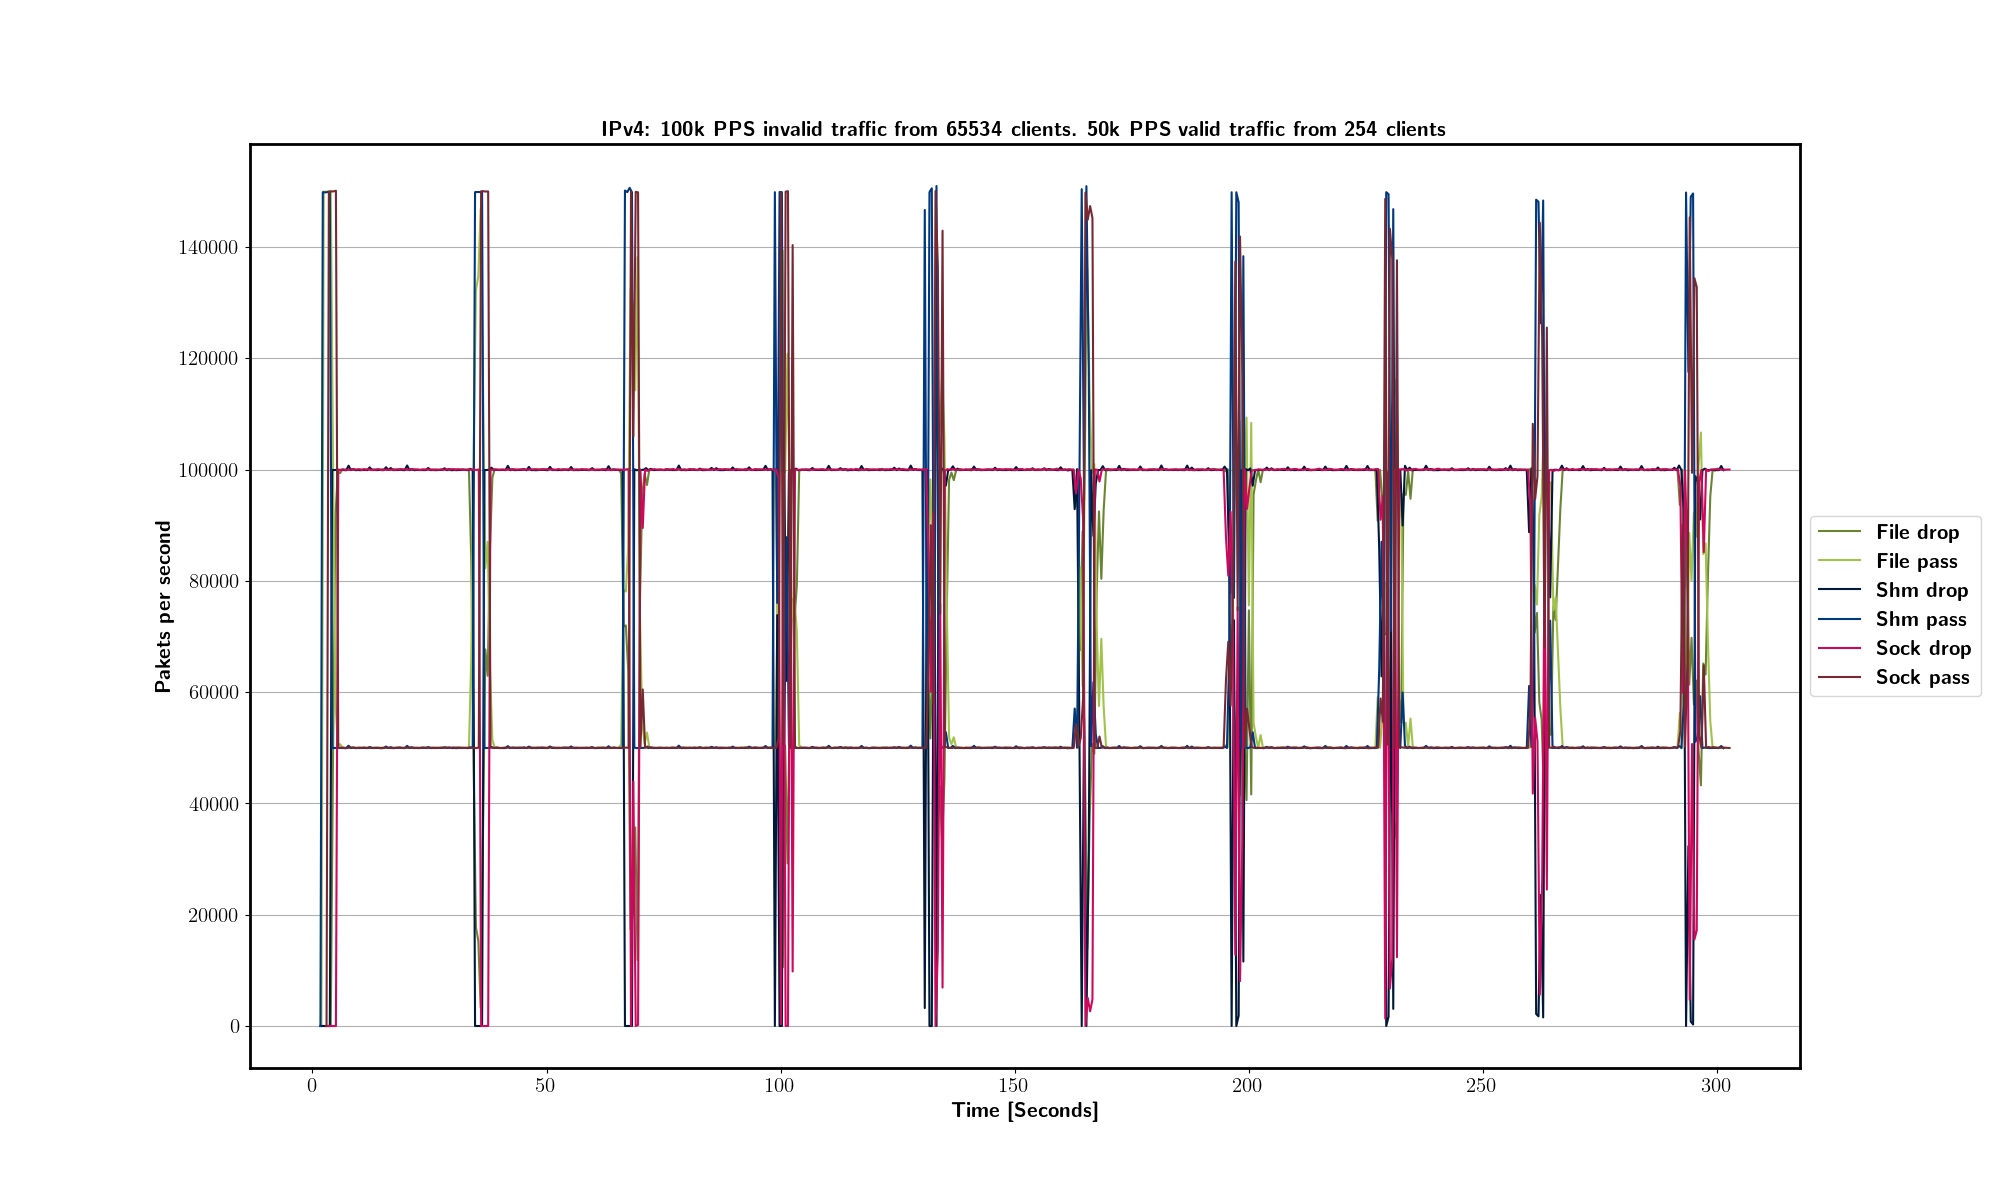
\includegraphics[width=1.2\textwidth]{images/IPv4_100k_65534_1.png}}
	\end{tabular}
	\begin{tabular}{llllll}
		\toprule
		\textbf{IPC type} & \textbf{Packets dropped [$10^6$]} & \textbf{Packets passed [$10^6$]} & \textbf{Relative drop [\%]} & \textbf{Log messages [$10^6$]} & \textbf{CPU [seconds]} \\ \midrule 
		File & 27,84 & 17,16 & 99,29900071 & 16,81 & 04.95 \\
        Shm & 28,03 & 16,97 & 100,0000036 & 16,97 & 05.94 \\
        Sock & 28,02 & 16,98 & 99,93706566 & 16,96 & 57.90 \\
	\bottomrule
	\end{tabular}
	\caption[Simplefail2ban, IPv4, 100k \ac{PPS}, 65534 malicious clients]{Total packets sent: 45m. Best case drop rate: 93,4466\%}
	\label{fig:data:ipv4:100k:65534}
\end{figure}

This trend somewhat continues in \ref{fig:data:ipv4:10m:65534}.
Again, the graph plotting the number of dropped and passed packets is not definitive.
Instead, a clear difference in performance is once again visible in CPU time.
The \texttt{relative drop} reveals that the shared memory IPC is performing best.
This is also supported by the lower number of packets passed to the kernel.

\begin{figure}[!h]
	\centering
	\scriptsize
	\begin{tabular}{c}
    	\centerline{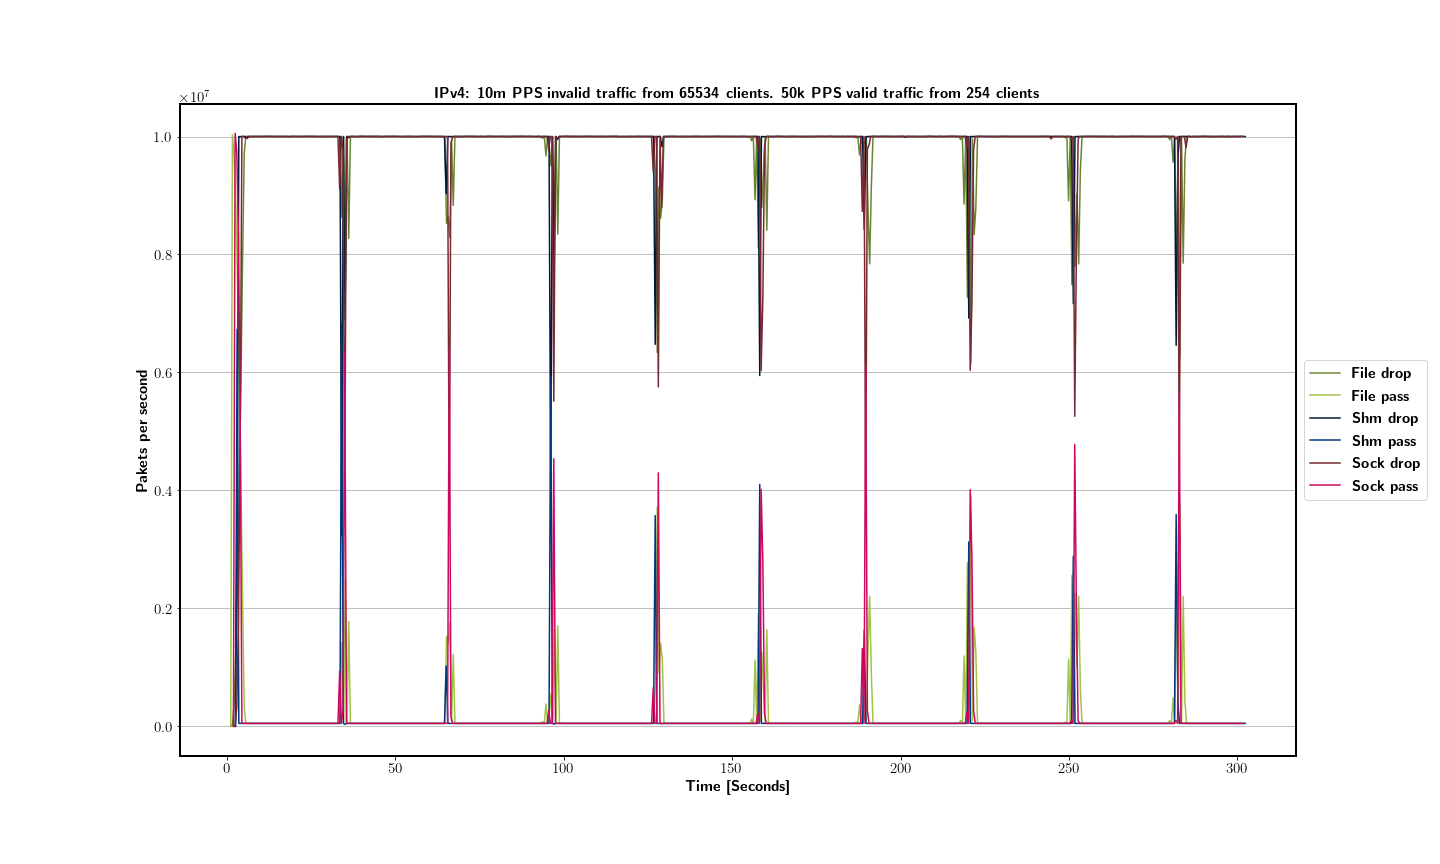
\includegraphics[width=1.2\textwidth]{images/IPv4_10m_65534_1.png}}
	\end{tabular}
	\begin{tabular}{llllll}
		\toprule
		\textbf{IPC type} & \textbf{Packets dropped [$10^8$]} & \textbf{Packets passed [$10^6$]} & \textbf{Relative drop [\%]} & \textbf{Log messages [$10^6$]} & \textbf{CPU [seconds]} \\ \midrule 
		File & 29,40 & 75,07 & 98,05973977 & 17,51 & 09.69 \\
        Shm & 29,75 & 37,49 & 99,21848407 & 20,02 & 16.86 \\
        Sock & 29,50 & 61,81 & 98,39458207 & 17,13 & 76.00 \\
	\bottomrule
	\end{tabular}
	\caption[Simplefail2ban, IPv4, 10m \ac{PPS}, 65534 malicious clients]{Total packets sent: 3015m. Best case drop rate: 99,934466\%}
	\label{fig:data:ipv4:10m:65534}
\end{figure}



Even with 30m invalid PPS, as seen in \ref{fig:data:ipv4:30m:65534}, all IPC types successfully defend against the DoS attack.
The fact that the file IPC type outperforms the socket IPC type in terms of \texttt{relative drop} rate is especially noteworthy.
File mode also outperforms shared memory and socket mode on CPU usage, which was not expected.
With the high rate of incoming traffic during a ban cycle, the application udp\_server had to wait on the IPC to be able to submit more log messages to Simplefail2ban.
This resulted the system being unable to submit a substantial number of packets to udp\_server.
While not explicitly documented in this thesis, these number are available in the repository\cite{git:repoOfThesis} of this thesis.
The difference in log messages created by udp\_server and number of passed packets correlates exactly with this observation.
Measuring the number of packets unable to be submitted to udp\_server was done by checking the file \texttt{/proc/net/udp6} on the DUT.

\begin{figure}[!h]
	\centering
	\scriptsize
	\begin{tabular}{c}
    	\centerline{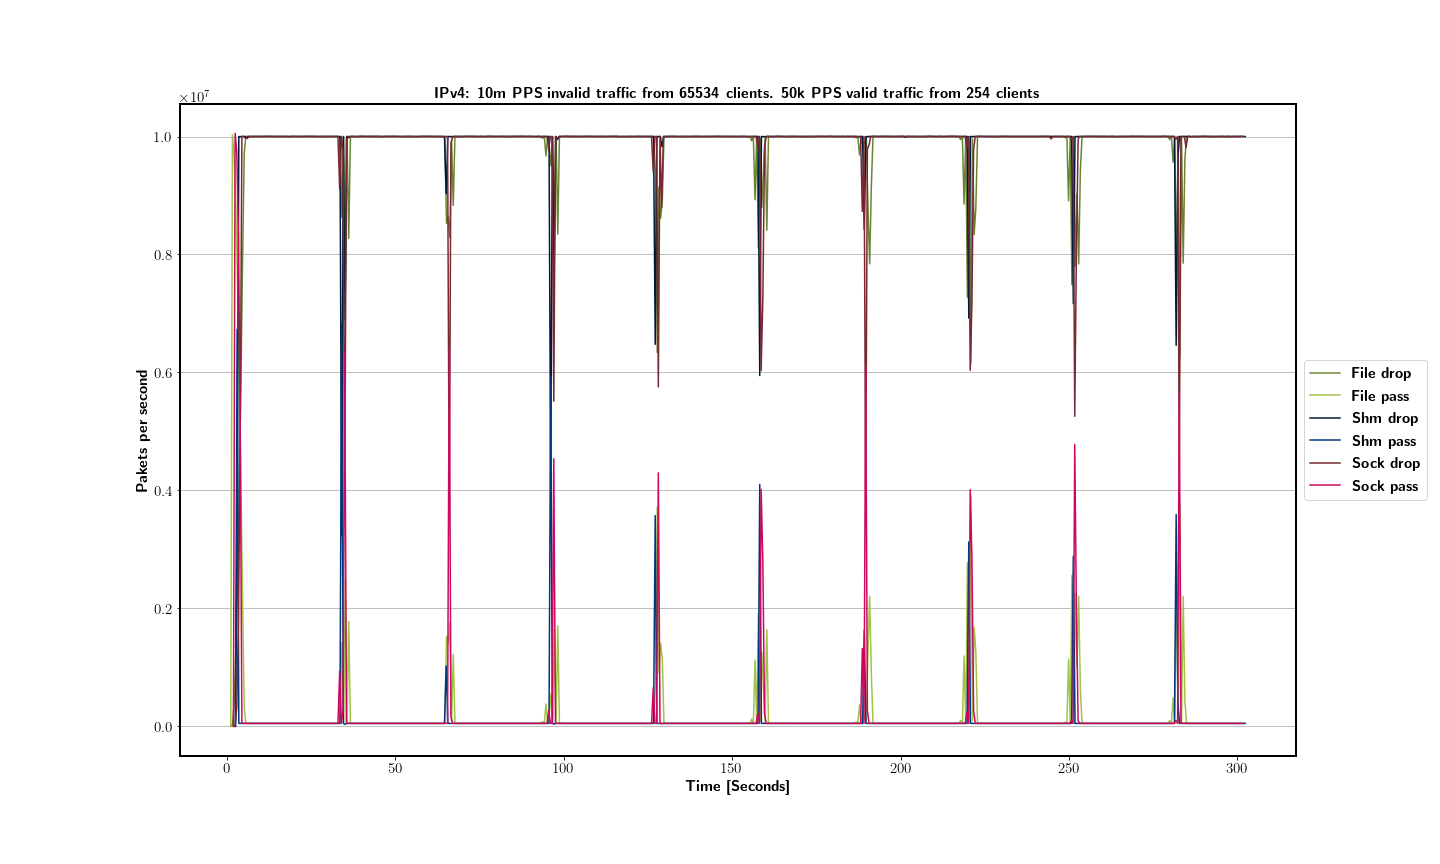
\includegraphics[width=1.2\textwidth]{images/IPv4_10m_65534_1.png}}
	\end{tabular}
	\begin{tabular}{llllll}
		\toprule
		\textbf{IPC type} & \textbf{Packets dropped [$10^8$]} & \textbf{Packets passed [$10^6$]} & \textbf{Relative drop [\%]} & \textbf{Log messages [$10^6$]} & \textbf{CPU [seconds]} \\ \midrule 
		File & 87,75 & 159,82 & 97,52375345 & 17,48 & 16.55 \\
        Shm & 88,30 & 87,23 & 98,13105047 & 21,39 & 39.08 \\
        Sock & 87,45 & 139,42 & 97,18179422 & 16,92 & 138.85 \\
	\bottomrule
	\end{tabular}
	\caption[Simplefail2ban, IPv4, 10m \ac{PPS}, 65534 malicious clients]{Total packets sent: 9015m. Best case drop rate: 99,97815533\%}
	\label{fig:data:ipv4:30m:65534}
\end{figure}
